\chapter{DHCP, NAT e IPv6}

% ══════════════════════════════════════════════════════════════
\section{L'assegnazione degli indirizzi IP}
% ══════════════════════════════════════════════════════════════

Ora sappiamo scoprire dove una rete è rotta. Non ci siamo mai chiesti da dove venga l'indirizzo di questa macchina:
nessuno l'ha scritto. È stato \textbf{chiesto}, concesso per un tempo limitato, e domani può essere un altro. L'altra
domanda è quella in cui le tracce continuavano a inciampare: un'intera rete che vive dietro un solo indirizzo pubblico. Il
protocollo che distribuisce gli indirizzi, la traduzione che fa servire una casa da un indirizzo, e il successore di IPv4
stanno insieme: esistono tutti e tre perché trentadue bit non bastavano, e non bastano da trent'anni.

Un blocco di indirizzi non è una configurazione: qualcuno deve ancora dare un indirizzo a ciascuna interfaccia. Un
amministratore di sistema può farlo in due modi:

\begin{itemize}
    \item \textbf{manualmente}: scrivendo indirizzo, maschera e gateway nella macchina (indirizzo \emph{statico}). È così che
          si configurano le interfacce dei router;
    \item \textbf{automaticamente}: è la rete ad assegnare un indirizzo libero a chiunque arrivi. È così che si configurano
          gli host.
\end{itemize}

Fare gli host a mano significa tenere una lista di quali indirizzi sono liberi e non sbagliarla mai; e non sopravvive al
movimento: un portatile portato da un'aula a una biblioteca a un'aula magna ha bisogno di un indirizzo nuovo in ciascun posto.
Il modo automatico è un protocollo, e gira su ogni macchina di quest'aula: il \textbf{Dynamic Host Configuration Protocol}
(DHCP).

\dfn{DHCP}{
    Il \textbf{DHCP} assegna automaticamente a un host che si collega alla rete le informazioni necessarie per
    usarla: oltre all'\textbf{indirizzo IP}, la \textbf{subnet mask}, l'indirizzo del \textbf{gateway predefinito}
    (per uscire dalla rete) e quello del \textbf{server DNS locale}. È \emph{plug-and-play} (o \emph{zeroconf}), ed è quello
    che si usa nelle nostre case.
}

Un indirizzo da solo non porta una macchina da nessuna parte. Le quattro cose arrivano insieme: l'indirizzo e la maschera
(quali destinazioni sono sulla mia subnet e quali no), il router del primo salto (dove deve andare tutto ciò che non è sulla
mia subnet) e il resolver DNS locale (senza il quale ogni nome che l'utente scrive è irrisolvibile).

% ══════════════════════════════════════════════════════════════
\section{Il funzionamento del DHCP}
% ══════════════════════════════════════════════════════════════

Il DHCP è un protocollo \textbf{client-server}: un host appena arrivato (client) contatta il server DHCP per ricevere
la configurazione di rete. Il servizio può essere offerto da un computer o, in una casa quasi sempre, dal router stesso.
Gira su UDP, porta \textbf{67} al server e \textbf{68} al client: formalmente è un protocollo di \textbf{livello
applicativo}. Vale un momento di riflessione: ciò che configura il livello di rete sta in cima alla pila e lo usa come
qualsiasi altra applicazione.

Riprendiamo l'esempio delle tre subnet collegate da un router, e supponiamo che la subnet di destra
(\texttt{223.1.2.0/24}) abbia un server DHCP: quando un nuovo host entra nella rete, ``contratta'' il proprio indirizzo
con il server. L'aggiunta di un host avviene in quattro passi (ricordati spesso con l'acronimo \textbf{DORA}):

\begin{figure}[H]
\centering
\begin{minipage}{0.34\linewidth}\centering
  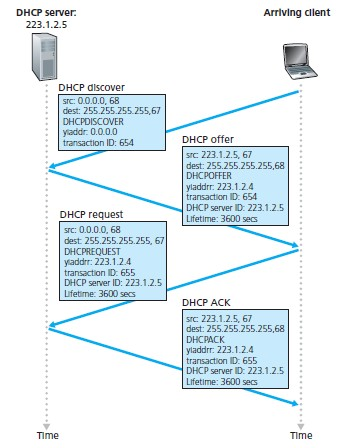
\includegraphics[width=0.9\linewidth]{cap15/dhcp_messaggi.png}
\end{minipage}\hfill
\begin{minipage}{0.62\linewidth}
\begin{enumerate}
  \item \textbf{Discover} --- ricerca del server: il nuovo host invia in \textbf{broadcast} un messaggio \emph{DHCP discover}
        (UDP, porta \textbf{67}) per trovare un server DHCP.
        \begin{itemize}
          \item IP destinazione: \texttt{255.255.255.255} (broadcast);
          \item IP sorgente: \texttt{0.0.0.0} (``questo host'', che non ha ancora un indirizzo);
          \item un identificativo di transazione casuale.
        \end{itemize}
  \item \textbf{Offer} --- offerta: poiché possono esserci più server, ogni server che riceve il discover risponde con un
        messaggio in broadcast (porta \textbf{68}) che offre una possibile configurazione (campo \texttt{yiaddr}, \emph{Your
        Internet ADDRess}). IP destinazione \texttt{255.255.255.255}, IP sorgente quello del server (\texttt{223.1.2.5}).
  \item \textbf{Request} --- richiesta: il client sceglie un'offerta tra quelle ricevute e la accetta ``facendo l'eco''
        del messaggio di offerta.
  \item \textbf{ACK} --- conferma: il server conferma la transazione con un messaggio finale.
\end{enumerate}
\end{minipage}
\caption{I quattro messaggi del DHCP (da Kurose).}
\end{figure}

Un \textbf{identificativo di transazione} lega insieme i quattro messaggi: nessuno di loro è indirizzato a qualcuno in
particolare.

\warning{Indirizzare un host che non ha un indirizzo}{
    Il client non ha un indirizzo. Che cosa va nel campo sorgente, e come può mai tornargli una risposta? Sorgente
    \texttt{0.0.0.0}, «questo host»; destinazione \texttt{255.255.255.255}, «tutti qui». Anche la risposta è in broadcast:
    nessuno dei due può ancora indirizzare l'altro, quindi gridano entrambi.
    \begin{itemize}
        \item A consegnare davvero quei due datagrammi è il livello sotto, che ha indirizzi suoi e un broadcast suo. Ogni
              interfaccia ne porta uno, fissato in fabbrica: non è un indirizzo IP, e non l'ha mai configurato nessuno.
        \item Un broadcast di subnet non viene inoltrato dai router, quindi tutto lo scambio è confinato a una subnet per
              costruzione: i quattro messaggi funzionano solo se il server sta sulla stessa subnet del client.
    \end{itemize}
}

\begin{figure}[H]
\centering
\begin{tikzpicture}[every node/.style={font=\scriptsize\sffamily}, node distance=0pt]
  \node[lay app, minimum width=3cm] (a) {Applicazione};
  \node[lay tra, minimum width=3cm, below=of a] (t) {Trasporto};
  \node[lay net, minimum width=3cm, below=of t] (n) {Rete};
  \node[lay link, minimum width=3cm, below=of n] (l) {Collegamento};
  \node[lay phy, minimum width=3cm, below=of l] (p) {Fisico};
  \draw[decorate, decoration={brace, amplitude=5pt, mirror}] ([xshift=-3pt]a.north west) -- node[left=6pt, align=right]{indirizzi IP:\\prefissi, maschere,\\subnet} ([xshift=-3pt]n.south west);
  \draw[decorate, decoration={brace, amplitude=5pt}] ([xshift=3pt]l.north east) -- node[right=6pt, align=left]{indirizzi di collegamento:\\un salto alla volta,\\niente subnet} ([xshift=3pt]l.south east);
  \draw[{Stealth[length=1.6mm]}-{Stealth[length=1.6mm]}, thick, netred] ([xshift=0.6cm]n.east) -- node[right, text=netred]{ARP} ([xshift=0.6cm]l.east |- l.north);
\end{tikzpicture}
\caption{Quale indirizzo appartiene a quale livello. Fra i due sta ARP: dato un indirizzo IP sulla propria subnet, produce
         l'indirizzo di collegamento da mettere sul frame. Lo smonteremo al livello di collegamento.}
\end{figure}

\subsection{Il DHCP relay agent}

\begin{itemize}
    \item Nell'esempio tutto funziona perché il server DHCP e l'host sono nella \textbf{stessa subnet}: i broadcast non
          attraversano i router.
    \item Se il server esiste ma sta in un'altra subnet, serve un \textbf{DHCP relay agent} che inoltri i messaggi DHCP (può
          farlo un router).
    \item Configurando il router come relay agent, anche gli host delle subnet \texttt{223.1.1.0/24} e \texttt{223.1.3.0/24}
          vengono serviti dal server DHCP della subnet \texttt{223.1.2.0/24}. Il relay raccoglie il discover e lo inoltra al
          server come normale datagramma unicast, aggiungendo l'indirizzo dell'interfaccia da cui è arrivata la richiesta:
          così il server sa da quale pool prendere l'indirizzo.
    \item Più server possono anche rispondere allo stesso discover: il client prende un'offerta e la nomina nella richiesta;
          le altre vengono rilasciate.
\end{itemize}

\subsection{Leggere che cosa ha dato il lease}

\begin{lstlisting}[language=bash, title={La configurazione ricevuta dal DHCP}]
$ ip addr show wlp9s0
2: wlp9s0: <BROADCAST,MULTICAST,UP,LOWER_UP> mtu 1500 state UP
    link/ether 34:e6:ad:f0:d5:11                       <- l'indirizzo del livello sotto
    inet 100.103.0.64/16 brd 100.103.255.255 scope global dynamic wlp9s0
       valid_lft 84532sec preferred_lft 84532sec
    inet6 fe80::47c4:ec38:2dc3:5d70/64 scope link
$ ip route
default via 100.103.0.1 dev wlp9s0 proto dhcp metric 600
100.103.0.0/16 dev wlp9s0 proto kernel scope link src 100.103.0.64
\end{lstlisting}

\begin{itemize}
    \item \texttt{dynamic} e \texttt{valid\_lft} lo dicono chiaramente: questo indirizzo è in prestito, e il conto alla
          rovescia è partito.
    \item Nemmeno la rotta di default è stata scritta a mano: \texttt{proto dhcp} dice chi l'ha messa lì.
    \item Tre delle quattro cose che servono a un host sono su questo schermo; la quarta, il resolver, è finita nel file
          \texttt{/etc/resolv.conf}.
\end{itemize}

\subsection{Un lease è temporaneo, e la connessione anche}

\begin{itemize}
    \item Un lease dura ore o giorni. Un client che vuole tenere il proprio indirizzo lo rinnova prima che il tempo scada; se
          non lo fa, l'indirizzo torna nel pool e viene offerto a qualcun altro.
    \item Se si sposta la macchina su un'altra subnet riceve un indirizzo diverso, che è l'unica cosa corretta da fare lì. Ma
          una connessione è nominata da quattro valori, e uno è appena cambiato: \textbf{ogni connessione aperta in quel momento
          è morta}.
    \item Niente a questo livello lo ripara. Tenere un indirizzo cambiando rete è un meccanismo separato, costruito per le reti
          cellulari.
\end{itemize}

% ══════════════════════════════════════════════════════════════
\section{Il problema della visibilità}
% ══════════════════════════════════════════════════════════════

Su Internet ci sono miliardi di dispositivi che dovrebbero avere un indirizzo IP univoco per essere raggiungibili da
chiunque. Ma è davvero necessario che \textbf{tutti} i dispositivi siano visibili a tutti? È una buona idea che la mia
stampante sia raggiungibile (e usabile) da chiunque su Internet? E una casa con quindici dispositivi non riceve quindici
indirizzi pubblici.

Avere tutti i dispositivi raggiungibili dall'esterno delle reti locali pone problemi evidenti:

\begin{itemize}
    \item gli indirizzi IP sono \textbf{finiti} (e gli IPv4 praticamente esauriti);
    \item se i dispositivi sono collegati localmente, spesso è irragionevole o indesiderabile esporli tutti su Internet;
    \item gli amministratori locali dovrebbero conoscere la struttura dei blocchi di indirizzi soprastanti per assegnare
          indirizzi liberi, cosa che spesso non dipende da loro (per esempio nelle reti di casa).
\end{itemize}

% ══════════════════════════════════════════════════════════════
\section{Il NAT}
% ══════════════════════════════════════════════════════════════

\dfn{Network Address Translation (NAT)}{
    Il servizio di \textbf{NAT} permette di \textbf{rimappare} gli indirizzi IP dei pacchetti di una rete in indirizzi
    diversi (\emph{network masquerading}). Si usa una \textbf{tabella di traduzione} che associa molte coppie
    indirizzo/porta locali (della LAN) a una coppia indirizzo/porta globale (della WAN). Il servizio può essere offerto
    dai router.
}

La rete locale mascherata si chiama \textbf{rete privata} (o \emph{realm} con indirizzi privati): gli indirizzi privati
sono validi \textbf{solo all'interno} della rete privata. Gli stessi indirizzi sono in uso in questo momento in un milione di
altre case, e due di loro non si incontreranno mai. Da fuori la scatola non è affatto un router: è una macchina con un
indirizzo, da cui l'altro nome, \emph{masquerading}.

\begin{figure}[H]
\centering
\begin{tikzpicture}[every node/.style={font=\footnotesize\sffamily}]
  \node (pc) at (0,1.4) {\icon[0.9cm]{pc}}; \node[left=0pt of pc, font=\scriptsize\ttfamily] {192.168.0.23};
  \node (lp) at (0,0) {\icon[1cm]{laptop}}; \node[left=0pt of lp, font=\scriptsize\ttfamily] {192.168.0.11};
  \node (ph) at (0,-1.4) {\icon[0.6cm]{smartphone}}; \node[left=0pt of ph, font=\scriptsize\ttfamily] {192.168.0.7};
  \node (r) at (4,0) {\icon[1.3cm]{router}}; \node[below=0pt of r, align=center] {router NAT};
  \foreach \n in {pc,lp,ph} \draw[wired] (\n) -- (r);
  \node[netcloud, minimum width=3cm] (i) at (9,0) {Internet};
  \draw[wired, line width=2pt] (r) -- node[above, font=\scriptsize\ttfamily] {203.0.113.221} (i);
  \draw[decorate, decoration={brace, amplitude=6pt, mirror}] (-1.8,-2.1) -- (4.6,-2.1) node[midway, below=7pt, text=netgreen!50!black] {rete privata: indirizzi 192.168.0.x};
  \draw[decorate, decoration={brace, amplitude=6pt, mirror}] (4.8,-2.1) -- (10.6,-2.1) node[midway, below=7pt, text=netblue] {per Internet c'è un solo indirizzo pubblico};
\end{tikzpicture}
\caption{Con il NAT tutti i dispositivi di casa escono verso Internet con lo stesso indirizzo pubblico del router.}
\end{figure}

\subsection{Un esempio di NAT}

\begin{figure}[H]
    \centering
    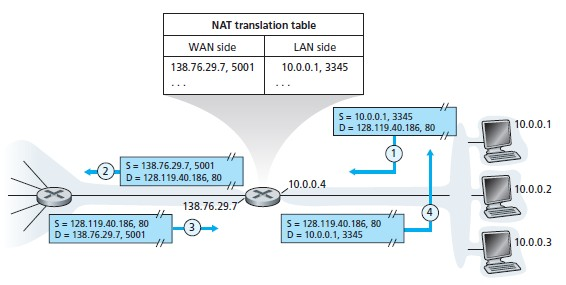
\includegraphics[width=0.7\linewidth]{cap15/nat_esempio.png}
    \caption{Un router NAT tra una rete privata 10.0.0.0/24 e Internet (da Kurose).}
\end{figure}

Le quattro interfacce della rete locale hanno indirizzi della subnet \texttt{10.0.0.0/24}; lato Internet il router ha un solo
indirizzo, \texttt{138.76.29.7}. Il router si comporta da ``passamessaggi'' che sovrascrive gli indirizzi secondo la tabella:

\begin{enumerate}
    \item L'host \texttt{10.0.0.1} invia un datagramma verso il server Web \texttt{128.119.40.186}, porta 80, usando la porta sorgente 3345.
    \item Il router NAT riceve il datagramma, sceglie una porta libera (\textbf{5001}) e \textbf{sostituisce} indirizzo
          e porta sorgente con la coppia \texttt{138.76.29.7, 5001}; poi aggiunge la riga alla tabella di traduzione.
    \item Il server risponde a \texttt{138.76.29.7, 5001}: per lui, la richiesta è arrivata dal router.
    \item Il router riceve la risposta, cerca \texttt{138.76.29.7, 5001} nella tabella e \textbf{riscrive} destinazione e porta con
          \texttt{10.0.0.1, 3345}, poi la inoltra nella LAN.
\end{enumerate}

\begin{table}[H]
\centering
\begin{tabular}{ll}
\toprule
\textbf{Lato WAN} & \textbf{Lato LAN} \\
\midrule
138.76.29.7, 5001 & 10.0.0.1, 3345 \\
138.76.29.7, 5002 & 10.0.0.2, 3345 \\
\dots & \dots \\
\bottomrule
\end{tabular}
\caption{La tabella di traduzione NAT: la seconda riga mostra perché serve una porta nuova.}
\end{table}

\warning{Perché il NAT cambia anche la porta}{
    Gli host non sanno nulla del traffico degli altri host: due host della LAN potrebbero scegliere \textbf{la stessa
    porta} sorgente (3345) nello stesso momento. Il NAT non può quindi riusare la porta iniziale, e ne assegna una nuova.
    Poiché la porta è di 16 bit, un NAT può gestire \textbf{oltre 60\,000 connessioni} contemporanee con un solo indirizzo IP
    pubblico; ed è anche il tetto, perché a quel confine finisce lo spazio delle porte, non l'indirizzo. E si noti che cosa fa
    il router per arrivarci: legge e riscrive un campo del livello di trasporto. Il server Web non lo scopre mai: risponde
    all'indirizzo e alla porta da cui è stato interpellato.
}

\subsection{Il limite del NAT}

\warning{Nessuno può cominciare da fuori}{
    Un host su Internet invia il primo datagramma a \texttt{10.0.0.1}. Che cosa ne fa il router? \textbf{Niente di utile}.
    Quella riga della tabella esiste solo perché la conversazione è stata avviata da dentro: senza riga, niente dice a quale
    delle macchine dietro il router sia destinato il datagramma.
    \begin{itemize}
        \item L'\textbf{inoltro delle porte} (\emph{port forwarding}) è una riga scritta a mano: tutto ciò che arriva su questa
              porta va a quella macchina. È la risposta per un servizio.
        \item La risposta generale è una famiglia di tecniche detta \textbf{NAT traversal}, in cui una terza macchina fuori
              aiuta due macchine interne a trovarsi. Ogni applicazione peer-to-peer deve farci i conti.
        \item E anche il server della chat: sulla propria LAN risponde, da fuori non esiste.
    \end{itemize}
}

\warning{Nemmeno il proprio indirizzo è nostro}{
    \texttt{100.103.0.64}, dalla configurazione letta poco fa, è uno degli indirizzi privati? Non sta in nessuno dei tre
    blocchi, e non è nemmeno un nostro indirizzo pubblico: appartiene a \texttt{100.64.0.0/10}, lo \textbf{spazio di indirizzi
    condiviso}, che i fornitori usano per numerare i propri clienti dietro un traduttore loro (\emph{carrier-grade NAT}).
    \begin{itemize}
        \item Allora le traduzioni sono due in fila, una in casa e una dal fornitore: niente fra quella macchina e Internet è
              suo.
        \item Il primo salto di una traccia da lì ha un indirizzo dello stesso blocco: un router del fornitore, non di Internet.
        \item Conseguenza: configurare il router di casa non basta per essere raggiungibili da fuori, perché il traduttore esterno
              non è nostro. È così che appare l'esaurimento degli indirizzi visto da un portatile.
    \end{itemize}
}

\subsection{Che cosa costa la traduzione}

\begin{itemize}
    \item \textbf{Le porte indirizzano processi}, non host: qui lo stesso campo serve a distinguere gli host, che è un lavoro
          diverso fatto con gli stessi bit.
    \item \textbf{I router sono dispositivi di livello di rete}, in teoria: questo legge e riscrive header di trasporto.
    \item E \textbf{tiene stato}: si perde la tabella e muore ogni conversazione che la attraversa. Un router che si limita a
          inoltrare non ha niente da perdere.
    \item L'argomento end-to-end dice che due host devono poter parlare senza che niente in mezzo alteri ciò che hanno detto;
          questo lo altera.
    \item E ha funzionato abbastanza bene da rimandare la vera risposta di venticinque anni: ci arriviamo alla fine del
          capitolo.
\end{itemize}

% ══════════════════════════════════════════════════════════════
\section{Gli indirizzi IP riservati}
% ══════════════════════════════════════════════════════════════

Perché gli amministratori locali possano organizzare una rete privata senza interferenze, per convenzione alcuni blocchi di
indirizzi sono \textbf{riservati}: ISP e ICANN non possono assegnarli a nessuna organizzazione.

\begin{table}[H]
\centering
\begin{tabular}{llp{7.5cm}}
\toprule
\textbf{Blocco} & \textbf{Intervallo} & \textbf{Uso} \\
\midrule
10.0.0.0/8 & 10.0.0.0 -- 10.255.255.255 & reti private \\
172.16.0.0/12 & 172.16.0.0 -- 172.31.255.255 & reti private \\
192.168.0.0/16 & 192.168.0.0 -- 192.168.255.255 & reti private (tipiche delle case) \\
127.0.0.0/8 & 127.0.0.0 -- 127.255.255.255 & ``questa macchina'' (\emph{loopback}), di solito 127.0.0.1 \\
100.64.0.0/10 & 100.64.0.0 -- 100.127.255.255 & spazio condiviso dei fornitori (\emph{carrier-grade NAT}) \\
0.0.0.0 & --- & rete corrente; per estensione, un indirizzo con la parte di host a 0 indica la rete \\
255.255.255.255 & --- & broadcast; per estensione, un indirizzo con la parte di host tutta a 1 è il broadcast della subnet \\
\bottomrule
\end{tabular}
\caption{Indirizzi IPv4 riservati.}
\end{table}

La riserva è necessaria perché gli indirizzi privati potrebbero coincidere con indirizzi pubblici, rendendo ambiguo
l'instradamento dentro la rete. Nessun registro li assegna mai: sono tenuti da parte proprio perché ogni rete privata possa
usarli nello stesso momento. Un router di Internet pubblica scarta un datagramma diretto a uno di loro: là fuori non c'è un
posto simile a cui mandarlo. Per sapere chi è acceso in una subnet privata si usano \texttt{ping} e \texttt{nmap -sn}, visti
nel capitolo precedente.

% ══════════════════════════════════════════════════════════════
\section{Esempio completo: configurare una LAN}
% ══════════════════════════════════════════════════════════════

Vogliamo creare una nuova rete locale (LAN) dentro una rete più grande preesistente (WAN). L'amministratore della WAN
ci fornisce:

\begin{itemize}
    \item l'indirizzo della WAN: \texttt{150.100.0.0/16};
    \item l'indirizzo del gateway che porta all'esterno (WAN/Internet): \texttt{150.100.50.1};
    \item un indirizzo libero per la nostra rete: \texttt{150.100.50.10}.
\end{itemize}

Useremo un router con NAT e decidiamo che la nuova LAN avrà indirizzo \texttt{192.168.1.0/24} (riservato alle reti private).

\begin{figure}[H]
\centering
\begin{tikzpicture}[every node/.style={font=\footnotesize\sffamily}]
  \node[netcloud, minimum width=2.8cm] (inet) at (0,3.2) {Internet};
  \node[draw=netblue, thick, rounded corners, fill=cloudbg, minimum width=7cm, minimum height=2.2cm] (wan) at (0,0.8) {};
  \node[anchor=north east, text=netblue] at (wan.north east) {WAN \texttt{150.100.0.0/16}};
  \node (rw) at (-1.8,1.0) {\icon[1.1cm]{router}}; \node[below=-1pt of rw, align=center, font=\scriptsize\sffamily] {router WAN\\\texttt{150.100.50.1}};
  \draw[wired, line width=2pt] (inet) -- (rw);
  \node[draw=netgreen!70!black, thick, rounded corners, fill=netgreen!8, minimum width=7cm, minimum height=2.6cm] (lan) at (0,-2.4) {};
  \node[anchor=south east, text=netgreen!50!black] at (lan.south east) {LAN \texttt{192.168.1.0/24}};
  \node (rl) at (-1.8,-1.6) {\icon[1.1cm]{router}};
  \node[anchor=west, font=\scriptsize\ttfamily, text=netblue] at (-1.2,-0.9) {WAN: 150.100.50.10};
  \node[anchor=west, font=\scriptsize\ttfamily, text=netgreen!50!black] at (-1.2,-1.8) {LAN: 192.168.1.1};
  \draw[wired] (rw) -- (rl);
  \node (h1) at (-2.3,-3.2) {\icon[0.8cm]{laptop}}; \node[right=0pt of h1, font=\scriptsize\ttfamily, align=left] {192.168.1.100\\(DHCP)};
  \node (h2) at (1.2,-3.2) {\icon[0.8cm]{pc}}; \node[right=0pt of h2, font=\scriptsize\ttfamily, align=left] {192.168.1.10\\(manuale)};
  \draw[wired] (rl) -- (h1); \draw[wired] (rl) -- (h2);
\end{tikzpicture}
\caption{La LAN da configurare: il router locale ha un'interfaccia nella WAN e una nella LAN.}
\end{figure}

\subsection{1. Il lato WAN del router}

Il router locale ha \textbf{due interfacce}, una verso la WAN e una verso la LAN. Sul lato WAN vanno impostati:

\begin{itemize}
    \item l'indirizzo del router nella WAN: \texttt{150.100.50.10};
    \item la subnet mask della WAN: \texttt{255.255.0.0};
    \item il gateway: \texttt{150.100.50.1};
    \item uno o più server DNS.
\end{itemize}

Vista dalla rete in cui entra, il router è solo un altro host: un'interfaccia, un indirizzo, e i quattro campi sono le
quattro cose di cui ogni host ha bisogno. È \textbf{statico} perché l'amministratore ci ha dato un indirizzo fisso; se la
WAN avesse un server DHCP, questa scatola sarebbe un client da un lato e un server dall'altro.

\begin{figure}[H]
    \centering
    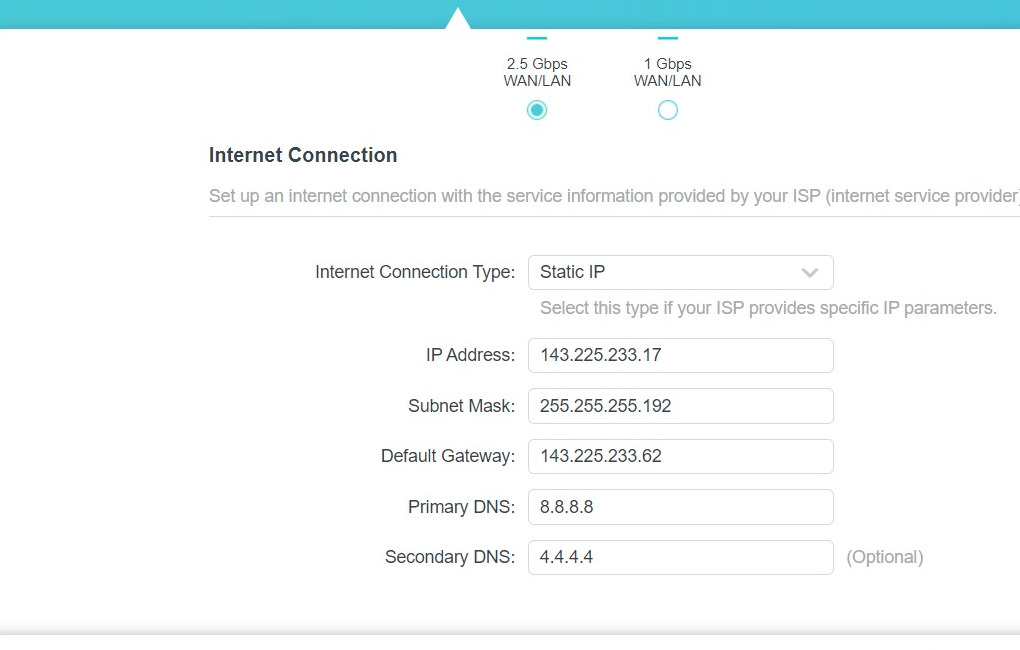
\includegraphics[width=0.6\linewidth]{cap15/config_wan.png}
    \caption{La pagina di configurazione ``Internet'' (lato WAN) di un router domestico: indirizzo statico, maschera, gateway e DNS (valori di un esempio reale, diversi da quelli del testo).}
\end{figure}

\subsection{2. Il lato LAN del router}

\begin{itemize}
    \item All'interfaccia LAN del router si dà un indirizzo della nuova rete: poiché la LAN è \texttt{192.168.1.0/24}, al router si
          assegna \texttt{192.168.1.1/24} (è consuetudine dare al router l'indirizzo \texttt{.1}).
    \item Se il router offre anche il DHCP, si specificano:
    \begin{itemize}
      \item il \textbf{pool di indirizzi} per gli host DHCP, per esempio da \texttt{192.168.1.100} a \texttt{192.168.1.250};
      \item il \textbf{lease time}: la durata dell'assegnazione, dopo la quale l'indirizzo può essere riusato (per esempio 120
            minuti: lease brevi riciclano gli indirizzi in fretta, lunghi sopravvivono a una macchina spenta);
      \item gateway e DNS da comunicare agli host: e il gateway che annuncia è se stesso.
    \end{itemize}
\end{itemize}

\begin{figure}[H]
    \centering
    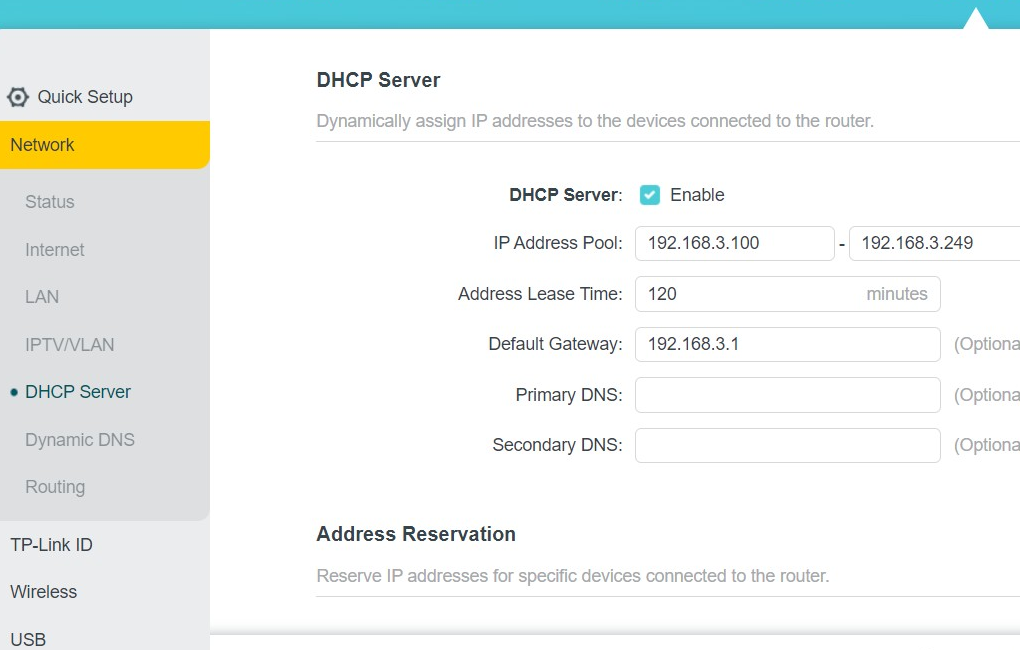
\includegraphics[width=0.6\linewidth]{cap15/config_lan.png}
    \caption{La configurazione del server DHCP del router: pool di indirizzi, lease time, gateway e DNS.}
\end{figure}

\subsection{3. Gli host}

Su un nuovo host (per esempio con Linux Mint) si può scegliere come configurare la connessione:

\begin{figure}[H]
\centering
\begin{minipage}{0.44\linewidth}\centering
  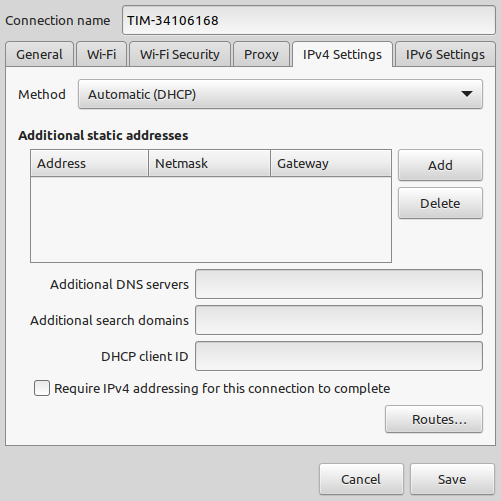
\includegraphics[width=0.85\linewidth]{cap15/host_dhcp.png}\\{\small (a) automatica (DHCP)}
\end{minipage}\hfill
\begin{minipage}{0.44\linewidth}\centering
  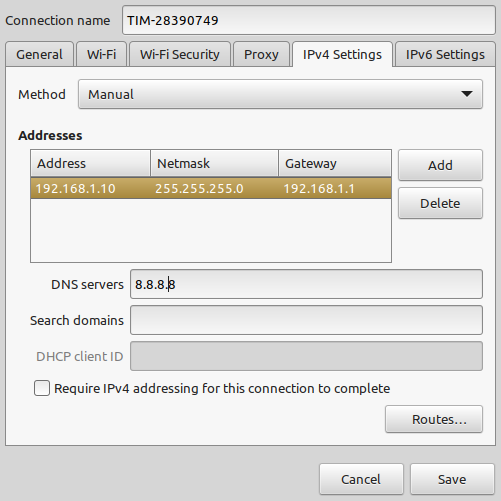
\includegraphics[width=0.85\linewidth]{cap15/host_manuale.png}\\{\small (b) manuale}
\end{minipage}
\caption{Configurazione della connessione su un host.}
\end{figure}

\begin{itemize}
    \item \textbf{Automatica (DHCP)}: l'host riceve dal DHCP un indirizzo tra \texttt{192.168.1.100} e \texttt{192.168.1.250}.
    \item \textbf{Manuale}: bisogna conoscere la configurazione della rete e gli indirizzi disponibili, e indicare
          l'\textbf{indirizzo dell'host} (statico, \textbf{fuori dal pool} del DHCP, per esempio \texttt{192.168.1.10}), la
          \textbf{subnet mask}, il \textbf{gateway} e uno o più \textbf{DNS}.
\end{itemize}

Gli host collegati inviano i loro pacchetti al router locale, senza sapere nulla della WAN esterna; il router locale è
configurato per inoltrarli al router della WAN, e da lì eventualmente a Internet.

\warning{Indirizzi manuali fuori dal pool}{
    Un indirizzo assegnato a mano deve stare \textbf{fuori} dall'intervallo del DHCP: \texttt{.10} sta sotto il pool, ed è
    voluto. Altrimenti prima o poi il DHCP lo offrirà a una macchina appena arrivata, e due interfacce della stessa subnet
    risponderanno allo stesso indirizzo (conflitto). Dopo la configurazione, niente distingue i due host: uno ha chiesto, l'altro
    è stato detto da qualcuno che sapeva. Tutto ciò che l'host invia va a \texttt{192.168.1.1}, che lo traduce e lo inoltra a
    \texttt{150.100.50.1}; l'host non sa nulla né dell'uno né dell'altro.
}

% ══════════════════════════════════════════════════════════════
\section{IPv6}
% ══════════════════════════════════════════════════════════════

All'inizio degli anni '90 l'IETF (organizzazione nata nel 1986) avviò lo sviluppo di un successore di IPv4, per
affrontare la \textbf{carenza di indirizzi} a 32 bit. IPv6 fu progettato per avere molti più indirizzi, ma fu anche
l'occasione per aggiornare altri aspetti di IPv4 sulla base dell'esperienza accumulata.

\begin{itemize}
    \item Due stime di chi lo stava misurando: gli indirizzi sarebbero finiti nel 2008, o nel 2018.
    \item \textbf{Febbraio 2011}: l'ultimo blocco non assegnato ha lasciato il pool centrale verso un registro regionale. Da
          allora i registri razionano.
    \item La traduzione è gran parte del motivo per cui la scadenza continuava a spostarsi: non ha creato indirizzi, ha fatto
          servire più macchine da ciascuno.
\end{itemize}

\info{E IPv5?}{
    Il numero di versione 5 è stato speso per un protocollo sperimentale di streaming, \emph{Internet Stream Protocol} (ST,
    poi ST-2), che è stato abbandonato e non è mai stato pensato come successore di IPv4. Al successore è toccato il 6.
}

\subsection{I vantaggi di IPv6}

\begin{itemize}
    \item \textbf{Indirizzi molto più grandi}: da 32 a \textbf{128 bit}, cioè $2^{128} \approx 3{,}4\cdot 10^{38}$ indirizzi. Il mondo
          non resterà senza indirizzi: si potrebbe dare un indirizzo a ogni granello di sabbia del pianeta.
    \item \textbf{Header di lunghezza fissa}, 40 byte: alcuni campi di IPv4 sono stati eliminati o resi facoltativi, e i router
          elaborano i pacchetti più velocemente.
    \item \textbf{Etichettatura dei flussi} (\emph{flow labeling}): 20 bit che nominano un flusso di datagrammi che vogliono lo
          stesso trattamento (un video, per esempio, piuttosto che un trasferimento di posta). Che cosa sia esattamente un
          flusso è stato lasciato aperto dalla specifica, ed è rimasto aperto: il campo c'è per quando sarà deciso.
    \item \textbf{Anycast}: un tipo di indirizzo del tutto nuovo, «consegna questo a uno qualsiasi di un gruppo»: il mirror più
          vicino, il resolver più vicino.
\end{itemize}
Con $3{,}4 \cdot 10^{38}$ indirizzi nessuno progetterà mai più uno schema per risparmiarli.

\info{Come si scrive un indirizzo IPv6}{
    Sedici byte in decimale puntato sarebbero illeggibili: un indirizzo IPv6 si scrive come \textbf{8 gruppi di 4 cifre
    esadecimali} separati da due punti, per esempio \texttt{8000:0000:0000:0000:0123:4567:89AB:CDEF}.
    \begin{itemize}
        \item Gli \textbf{zeri iniziali} di un gruppo si possono omettere: \texttt{0123} diventa \texttt{123}.
        \item Una sequenza di gruppi tutti a zero si può sostituire con \texttt{::}, \textbf{una sola volta} per indirizzo: due
              volte e la lunghezza sarebbe ambigua. L'esempio diventa \texttt{8000::123:4567:89AB:CDEF}.
        \item Un indirizzo IPv4 si può scrivere dopo una coppia di due punti, come in \texttt{::192.31.20.46}.
        \item L'indirizzo di loopback è \texttt{::1}; la riga \texttt{fe80::} nella configurazione letta prima è un indirizzo
              di questo tipo (\emph{link-local}): quella macchina aveva un indirizzo IPv6 da sempre.
    \end{itemize}
}

\subsection{Il datagramma IPv6}

\begin{figure}[H]
    \centering
    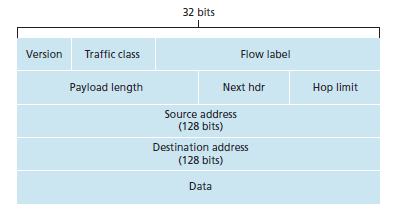
\includegraphics[width=0.55\linewidth]{cap15/ipv6_datagramma.png}
    \caption{Il datagramma IPv6: header fisso di 40 byte.}
\end{figure}

\begin{itemize}
    \item \textbf{Version} (4 bit): la versione, cioè 6.
    \item \textbf{Traffic class} (8 bit): come il TOS di IPv4, serve a dare priorità ai datagrammi (per esempio voce su IP rispetto a SMTP).
    \item \textbf{Flow label} (20 bit): identifica un flusso di datagrammi.
    \item \textbf{Payload length} (16 bit): numero di byte del payload (esclusi i 40 byte di header).
    \item \textbf{Next header} (8 bit): il protocollo superiore a cui consegnare i dati (TCP, UDP, \dots), come il campo protocollo di IPv4.
    \item \textbf{Hop limit} (8 bit): il time-to-live, decrementato a ogni inoltro.
    \item \textbf{Indirizzi sorgente e destinazione} (128 + 128 bit).
    \item \textbf{Data}: il payload.
\end{itemize}

Nella prima parola versione, classe di traffico e flow label (quale protocollo, quale priorità, quale flusso); nella seconda
lunghezza del payload, next header e hop limit (quanto segue, che cos'è, quanto lontano può ancora andare); poi i due
indirizzi, sedici byte ciascuno: trentadue dei quaranta byte sono indirizzi, e nessun campo misura un header di dimensione
fissa.

\begin{table}[H]
\centering
\begin{tabular}{l l l}
\toprule
\textbf{IPv4} & \textbf{IPv6} & \\
\midrule
time to live    & hop limit      & lo stesso contatore, chiamato onestamente \\
protocol        & next header    & gli stessi valori, e un compito in più \\
type of service & traffic class  & lo stesso compito \\
total length    & payload length & non conta più l'header \\
\bottomrule
\end{tabular}
\caption{Stesso compito, nome nuovo. Il cambio non è cosmetico: il time to live era specificato in secondi e usato da tutti
         come conteggio dei salti, e il nuovo nome dice che cos'è. \emph{Next header} nomina il protocollo di trasporto
         oppure punta al primo di una catena di header facoltativi; \emph{payload length} conta ciò che segue l'header, quindi
         un payload può essere di 65\,535 byte pieni.}
\end{table}

\subsection{Cosa manca rispetto a IPv4}

\begin{itemize}
    \item \textbf{Campi della frammentazione}: IPv6 non permette frammentazione e riassemblaggio nei router intermedi, ma solo negli
          host. Se un router riceve un datagramma IPv6 troppo grande da inoltrare, lo \textbf{scarta} e rimanda al mittente un
          messaggio di errore ``\emph{Packet Too Big}''; il mittente rinvia i dati con datagrammi più piccoli.
    \item \textbf{Checksum dell'header}: richiede tempo in ogni router ed è ridondante, perché i protocolli di collegamento di
          solito controllano già l'intero pacchetto (e TCP/UDP controllano i propri dati).
    \item \textbf{Opzioni}: non fanno più parte dell'header standard; alcune si possono indicare nel campo \emph{next header}
          (accanto agli identificativi di TCP/UDP), come header di estensione, dove un router a cui non interessano li salta.
\end{itemize}
Tutto ciò che è stato tolto è stato tolto per una sola ragione: era lavoro fatto a ogni salto, da ogni router, su ogni
datagramma.

% ══════════════════════════════════════════════════════════════
\section{Dalla IPv4 alla IPv6}
% ══════════════════════════════════════════════════════════════

C'è un grosso problema: IPv6 \textbf{non è retrocompatibile}. I sistemi che capiscono solo IPv4 non sanno gestire i datagrammi IPv6.
Come può Internet adottare IPv6?

\begin{itemize}
    \item \textbf{Flag day}: a una certa data e ora tutte le macchine di Internet vengono spente e aggiornate da IPv4 a IPv6. Si
          fece una volta, per il passaggio a TCP, su una rete di qualche centinaio di macchine, e fu doloroso già allora: con
          miliardi di dispositivi e nessuno che li governi tutti, l'idea non è nemmeno discutibile.
    \item \textbf{Doppio stack}: ciò che si fa invece è far convivere i due protocolli. La maggior parte delle macchine oggi li
          esegue entrambi e sceglie per destinazione, ed è per questo che la configurazione letta sopra aveva un indirizzo di
          ciascun tipo.
    \item \textbf{Tunneling}: dove un tratto del percorso parla solo IPv4, i datagrammi vanno trasportati attraverso in qualche
          modo. Due router IPv6 con solo IPv4 in mezzo: l'intero datagramma IPv6 diventa il payload di un datagramma IPv4
          indirizzato all'altro capo.
\end{itemize}

\begin{figure}[H]
\centering
\begin{tikzpicture}[every node/.style={font=\scriptsize\sffamily}]
  \foreach \x/\n/\c in {0/A/lnet, 2.6/B/lnet, 5.2/C/lphy, 7.8/D/lphy, 10.4/E/lnet, 13/F/lnet} {
    \node (\n) at (\x,0) {\icon[0.9cm]{router}}; \node[above=-2pt of \n] {\n};
  }
  \node[below=0pt of A] {IPv6}; \node[below=0pt of B] {IPv6/v4}; \node[below=0pt of C] {IPv4}; \node[below=0pt of D] {IPv4}; \node[below=0pt of E] {IPv6/v4}; \node[below=0pt of F] {IPv6};
  \foreach \a/\b in {A/B, B/C, C/D, D/E, E/F} \draw[wired] (\a) -- (\b);
  \draw[very thick, netorange, rounded corners, dashed] (2.4,-1.2) rectangle (10.6,0.9);
  \node[text=netorange, font=\footnotesize\bfseries\sffamily] at (6.5,1.1) {tunnel};
  \node[field, fill=lnet!60, minimum width=1.6cm] at (1.3,-1.8) {datagramma IPv6};
  \node[field, fill=lphy!80, minimum width=1.1cm] (h4) at (5.6,-1.8) {header IPv4};
  \node[field, fill=lnet!60, minimum width=1.6cm, right=0pt of h4] {datagramma IPv6};
  \node[field, fill=lnet!60, minimum width=1.6cm] at (11.7,-1.8) {datagramma IPv6};
\end{tikzpicture}
\caption{Tunneling: B incapsula il datagramma IPv6 in un datagramma IPv4 per attraversare C e D; E lo estrae. I router in
         mezzo inoltrano un normale datagramma IPv4 e non scoprono mai che cosa trasportano; il numero \textbf{41} nel campo
         protocollo dell'header IPv4 dice all'altro capo che cosa c'è dentro, esattamente come 6 dice TCP e 17 UDP. Niente
         viene tradotto: ciò che esce è ciò che è entrato.}
\end{figure}

\subsection{Perché questo livello è quello difficile da cambiare}

\begin{itemize}
    \item L'adozione è stata lenta per un decennio, poi ha cominciato a muoversi: nel 2020 circa un quarto dei client che
          raggiungevano Google lo faceva su IPv6. Le reti mobili hanno spinto più di tutti: un operatore che numera milioni di
          telefoni non ha altre opzioni.
    \item La lezione generale: il livello di rete è l'unica cosa su cui ogni macchina di Internet deve essere d'accordo, e
          l'accordo è la parte costosa. Il livello applicativo cambia di continuo (HTTP è stato riscritto due volte nel
          frattempo) perché ogni volta devono essere d'accordo solo due estremi.
    \item Venticinque anni, per un protocollo il cui unico cambiamento serio è la larghezza di un indirizzo.
\end{itemize}

\Needspace{20\baselineskip}
% ══════════════════════════════════════════════════════════════
\section{Riepilogo}
% ══════════════════════════════════════════════════════════════

\riepilogo{
\begin{itemize}
    \item Il \textbf{DHCP} assegna automaticamente indirizzo, maschera, gateway e DNS con quattro messaggi: discover, offer,
          request, ACK (broadcast, porte UDP 67/68); oltre le subnet serve un relay agent. Tutto arriva in prestito (lease), e
          cambiando subnet le connessioni aperte muoiono con il vecchio indirizzo.
    \item Il \textbf{NAT} fa uscire una rete privata con un solo indirizzo pubblico, riscrivendo indirizzi e porte secondo una
          tabella; funziona solo per conversazioni avviate da dentro (le altre richiedono port forwarding o NAT traversal),
          mette stato in mezzo alla rete, ed è ciò che ha fatto durare IPv4 così a lungo.
    \item Blocchi \textbf{riservati}: 10/8, 172.16/12, 192.168/16 (privati), 127/8 (loopback), 0.0.0.0, 255.255.255.255.
    \item \textbf{IPv6}: indirizzi a 128 bit, header fisso di 40 byte, flow label; niente frammentazione nei router, niente checksum,
          niente opzioni nell'header; transizione con doppio stack e \textbf{tunneling} (protocollo 41), senza una data di fine.
    \item Resta da chiedersi da dove vengono le righe di una forwarding table: è la prossima domanda.
\end{itemize}
}
